\documentclass[10pt,a4paper]{article}
\usepackage[margin=2cm]{geometry}
\usepackage{graphicx}
\usepackage{tabularx}
\usepackage{color}
\usepackage{caption}
\usepackage{subcaption}
\usepackage{tabu}
\usepackage{gensymb}
\usepackage{enumitem}
\usepackage{wrapfig}
\usepackage{algorithmic}
\usepackage{listings}

\captionsetup[figure]{labelfont=bf}
\captionsetup[table]{labelfont=bf}

\title{\vspace{-3em}Join Algorithms in SPARQL and their Scalability}
\author{pbqk24}
%\date{}

\begin{document}
	\maketitle
	
	\vspace{-3em}
	
	\section*{Abstract}
	
	The Semantic Web is an idea of the web as a network of data which can be processed by machines. One framework for storing information that fulfils this is the Resource Description Framework, RDF. This can be queried using a query language such as SPARQL, akin to SQL for relational databases. SPARQL implements several join algorithms to combine queries and yield more complex results. This project aims to investigate two of these join algorithms, and analyse their scalability with the number of join algorithms used and the limit imposed on the size of the result. The goal is to better inform decisions of which join algorithms to use by gathering data on their performance. The join algorithms were mainly compared by wall-clock running times, collected as an average over several queries to DBPedia, for different numbers of joins used and different LIMIT values. The results show a clear positive correlation between both factors and the running time of the query for both types of joins, to different extents. Potential areas for future investigation include considering scalability of combinations of different join algorithms, and comparisons to similar queries and databases in SQL.
	
	% Summarise the project, including algorithms compared, measuring criteria, and the main results
	\section*{Introduction}
	The Semantic Web originated as a vision by Tim Berners-Lee of a web composed of data that could be directly processed by computers. Much progress has been made on turning this vision into a reality: for example, as of 2016 there were 2740 datasets implementing the principles of the Semantic Web, compared to only 1091 in 2014 \cite{Bizer}. Most of these datasets use RDF to model the information and data stored in them. SPARQL is a query language for RDF, analogous to SQL for querying relational databases, which is used to retrieve data from RDF. Similarly to SQL, SPARQL implements several kinds of join algorithms in order to allow the combination of queries and data.
	
	As join algorithms are extensively used to build more complicated and useful queries, their implementation and efficiency is worthy of investigation. This will allow for analysis of the join algorithms, and the cost of using them in a query in terms of execution times. This project therefore investigates the scalability of two different join algorithms in SPARQL. The algorithms are compared in terms of scalability with the number of joins performed and the limit imposed on the number of results returned. This scalability is quantified in terms of wall-clock running time.
	
	% Set the scene, overview, motivation behind the work and choices
		% Brief overview of Semantic Web, RDF, SPARQL, their uses and why they are important
	% Overall description of what you did, main contributions
		% Analyse and compare the scalability of different join algorithms in SPARQL
	% How you are comparing algorithms, and how to measure the comparison
		% The algorithms are being compared in terms of their scalability, as well as their effect (i.e. what their effect is on the data/how they join data). This is measured in terms of wall-clock running time when ran on data on DBpedia. They are also compared to equivalent join operations in SQL
	
	\section*{Methodology}
	
	The first of the two join algorithms investigated is conjunction, the `.' operation in SPARQL. This takes two queries and returns only those result that are in the results of both queries, joining them by matching the values of the common variables. This algorithm is visualized in Figure \ref{inner_join}. This algorithm was chosen because it is exceedingly common in SPARQL, as it is used to combine several queries to place multiple constraints on the result. It therefore forms the building block of most complex queries.
		
	\begin{wrapfigure}{l}{0.3\textwidth}
		\vspace{-1em}
		\centering
		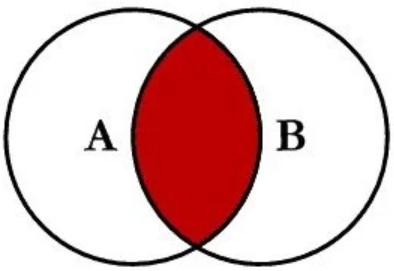
\includegraphics[width=0.3\textwidth]{figures/inner_join}
		\caption{Conjunction of two queries with `.', equivalent to inner join in SQL \cite{Moffatt}}
		\label{inner_join}
		\vspace{-1em}
	\end{wrapfigure}

	A query was designed that uses only this type of join in order to investigate its performance and scalability. This query is shown in Figure \ref{alg:inner_join} in the appendix. The query searches for a person who has a name, a gender, and a partner who also has a name and gender. The number of queries and joins used and the limit value were adjusted as desired for the investigation.
	
	\begin{wrapfigure}{r}{0.3\textwidth}
		\vspace{-1em}
		\centering
		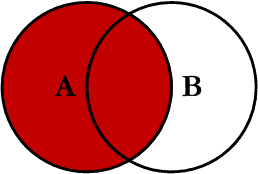
\includegraphics[width=0.3\textwidth]{figures/left_join}
		\caption{Effect of OPTIONAL in SPARQL queries, equivalent to left join in SQL \cite{Moffatt}}
		\label{left_join}
		\vspace{-1em}
	\end{wrapfigure}
	
	The second join algorithm implemented is OPTIONAL, which takes two queries and returns all results from the first query, with results from the second query added if they are found. This join is visualized in Figure \ref{left_join}. This join algorithm was chosen as it is commonly used in SPARQL queries, for example being used in up to 50\% of queries submitted to DBPedia \cite{Atre}. It is useful when querying RDF to retrieve data if it is found, but not place a requirement on it existing. For this join algorithm the difference between applying joins nested or sequentially was also investigated. Note that these two approaches are not equivalent. Both queries are included in Figure \ref{left_join_queries} in the appendix.
	
	The performance metrics for the join algorithms were gathered using yasgui.org, an online SPARQL query engine. Development and initial data gathering was mainly done using Python and the SPARQLWrapper library. Each query was performed 10 times on yasgui.org, with each execution being individually timed. Then, the top two results were removed to account for outliers due to networking reasons, and the rest were averaged. The full Python code used is attached in the appendix.
	
	These queries were designed to be simple to ensure a large amount of data would be available to allow investigation of higher LIMIT values. Scaling with numbers of queries used was chosen as a metric as it can measure the impact of using the join algorithm in complex queries. This could inform a decision to simplify a query, or divide it into multiple, simpler queries. Likewise scalability with the LIMIT value was chosen as this investigates the trade-off between performance and number of results to be returned. This could inform a decision to reduce the number of results to improve performance. Thus, both these metrics have direct applications for the design of SPARQL queries.
	
	% Describe the algorithms and implementation details
		% Basic algorithm: Retrieve all persons that have a name
		% Augmented with additonal joins (inner joins) to filter data further: require a gender, require a spouse, require the spouse's name, require the spouse's gender
		% Second algorithm: same properties, but using OPTIONAL, i.e. retrieve all persons, list their name if they have one, list their gender if they have one, list their spouse if they have one, list their spouse's name if they have one, list their spouse's gender if they have one
		% These were implemented using an online SPARQL query GUI (yasgui.org) to facilitate development and exploration of the data. Performance metrics were gathered by using Python and the SPARQLWrapper library to repeatedly query dbpedia and collect wall-clock running times. This allowed for easier automation and repetition of experiments to get more accurate averaged data.
	% Include what measures you will measure the methods on
		% The methods are measured on wall-clock running times. As previously mentioned, this is done for several combinations of different scaling parameters (number of joins performed, limit imposed on the result). In the case of several outer joins, the case of sequentially applied joins vs nested joins is also investigated
	% Explain your choices
		% Inner join was chosen as the first algorithm because it is very commonly used in SPARQL queries in order to combine several groups of triples, e.g. to place several constraints on the return values (e.g. return each person, the person must have a name, the person must have a gender).
		% Optional is also extremely commonly used (used in up to 50% of queries submitted to DBPedia (https://www.cs.ox.ac.uk/people/medha.atre/papers/sigmod2015-atre.pdf)). It allows queries to return data if it is present, but not enforce the data's existence as a constraint, and thus is extremely useful in the semi-structured world of RDF.
	
	\section*{Results}
	
	The results for the inner join algorithm are displayed in Figure \ref{fig:inner_join}. This graph shows a clear correlation between running time and the number of join algorithms used, and with the LIMIT value used. This is expected as the more join algorithms are used the more queries need to be executed and the results matched. Likewise, as the LIMIT value increases more results need to be selected and returned. These correlations hold for all values except for 3 joins and a LIMIT of 2000, which is higher than expected. This is likely an outlier caused by factors such as network connectivity or DBPedia load.
	
	\begin{figure}[h!]
		\centering
		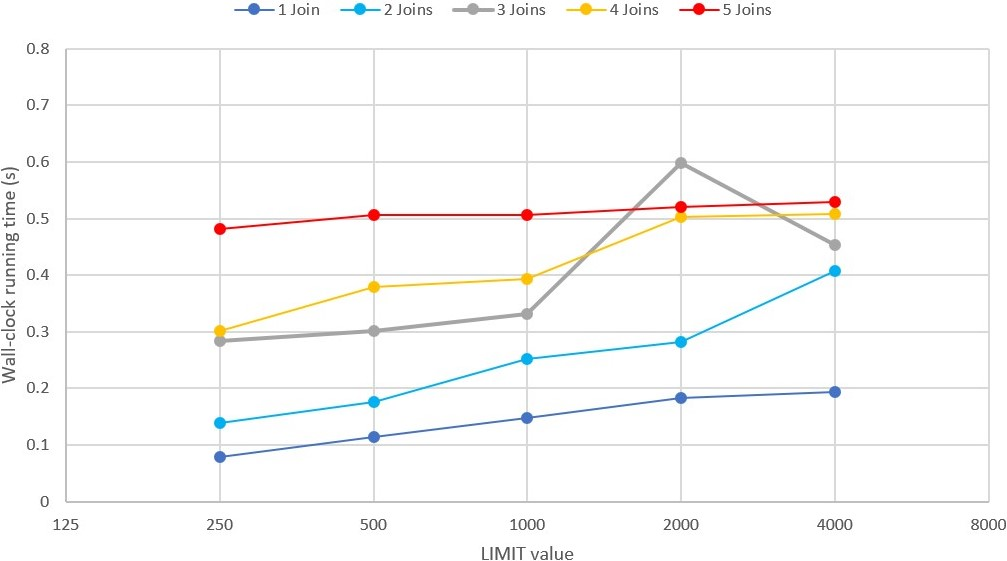
\includegraphics[width=0.8\textwidth]{figures/graph_inner_join}
		\caption{Wall-clock running times of inner join for varying numbers of joins performed and LIMIT values}
		\label{fig:inner_join}
	\end{figure}
	
	Notably, there is a much stronger correlation between running time and the number of joins than with the LIMIT value. This is likely because for each additional join algorithm added one additional query needs to be performed, and these results need to be matched against the rest. As the LIMIT value is increased the same number of queries and matchings are performed, and only the process of selecting values to be returned is lengthened. The data does, however, suggest that the LIMIT value used affects the scaling with multiple join algorithms. For a LIMIT value of 2000 there seems to be a linear increase in running time as more joins are used, while for a LIMIT of 4000 the increase decays as more joins are introduced.
	
	Figure \ref{fig:left_join} shows the results for the left join algorithm. There is no data for five joins, as this query resulted in a server timeout. Figure \ref{fig:seq_left_join}, which shows the results for left joins applied sequentially, displays a clear correlation between the running time and the LIMIT value, and a weaker correlation to the number of joins applied. This is very different from the inner join data. This is likely because the simple OPTIONAL joins used should be able to be optimised by the query engine to find as many results as requested first, and then execute the OPTIONAL queries only on this data, rather than the entire result of the first query, and still return correct results. This would explain the strong scaling with LIMIT value, as this increases the time taken for each query, and the weak scaling with numbers of joins performed. Again, this graph suffers from noise and some values which are likely to be outliers, such as the values for the query with three joins. As this entire query seems to have had lower running times than would be expected, this was likely caused by a temporary fall in server load or network activity.
	
	\begin{figure}[h!]
		\centering
		\begin{subfigure}[b]{0.46\textwidth}
			\hspace{-1cm}
			\centering
			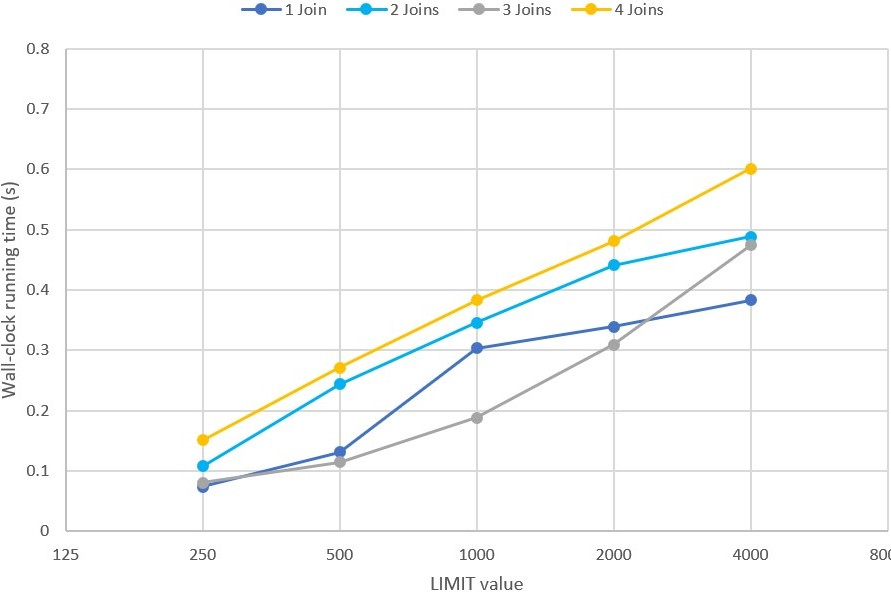
\includegraphics[width=1.1\textwidth]{figures/graph_sequential_left_join}
			\caption{Sequential Left Join}
			\label{fig:seq_left_join}
		\end{subfigure}
		\begin{subfigure}[b]{0.46\textwidth}
			\hspace{1cm}
			\centering
			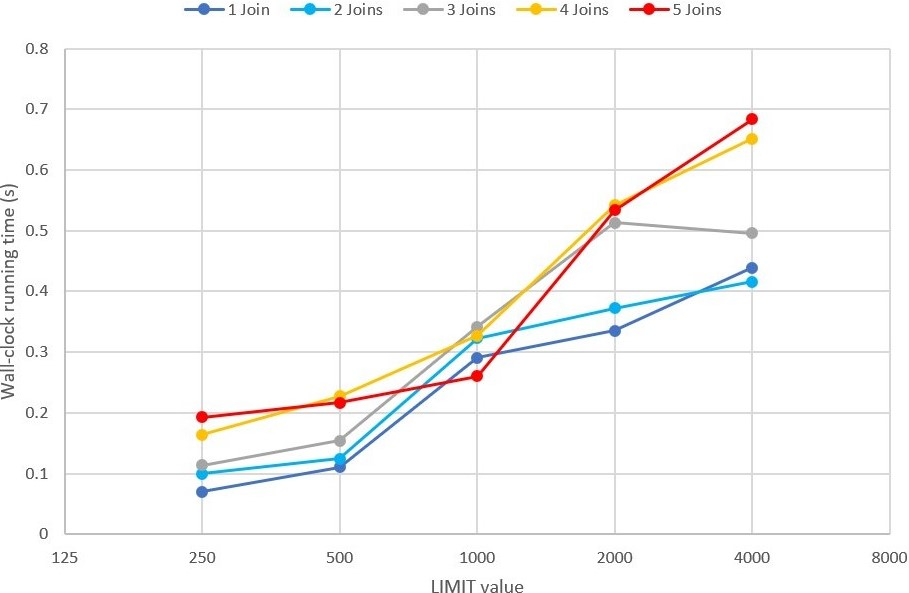
\includegraphics[width=1.1\textwidth]{figures/graph_nested_left_join}
			\caption{Nested Left Join}
			\label{fig:nested_left_join}
		\end{subfigure}
		\caption{Wall-clock running times of left join for varying numbers of joins performed and LIMIT values}
		\label{fig:left_join}
	\end{figure}

	The data gathered for the nested left join algorithms is shown in Figure \ref{fig:nested_left_join}. There is a correlation between running time and both LIMIT value and numbers of joins performed, but it is not as clear as for the other two experiments. In general, the data is very similar to that of the sequentially applied left joins, with the notable difference that the query with five left joins did not time out. Lastly, it is worth noting that the running times for the inner join queries were generally much higher for low LIMIT values than the queries with left joins, but lower or similar for higher LIMIT values, potentially caused by query optimisation as discussed previously.

	\section*{Conclusion}
	
	In conclusion, the scalability of join algorithms in SPARQL differs for each algorithm. The running time of inner join scales linearly with the number of queries performed, and only slightly with the LIMIT value imposed on the results, while both sequential and nested left joins exhibit the reverse. Compared to sequentially applied left joins, nested left joins are slightly faster at lower LIMIT values, but slower at higher values.
	
	There are several directions in which this project could be continued in the future or if given more time. First and foremost, more join algorithms could be investigated and compared to those included here to give a complete view of the join algorithms available in SPARQL. Another option is to investigate more complex scalability cases, such as using a combination of join algorithms, in order to produce more practical and directly relevant results. Also, the queries and join algorithms considered could be compared to similar queries and databases in SQL to compare the performance of SPARQL to SQL.
	
	The most likely first step for future expansion would be to gather data by querying a local database and tracking wall-clock running times on the server, rather than querying an online database with client-side timing. This would produce more accurate timing results, as the impact of network speed and load and database load would be removed from the timings. This would likely produce results more consistent with the expected outcome and the general trends found in this project.
	
	% What could you have done if you had more time
		% Investigate further/more complicated scalability cases, e.g. combination of inner and left joins.
		% Impact of query ordering on performance and scalability
		% Producing more accurate query wall-clock timings by querying a local database and tracking timings server-side, in order to remove impact of network speeds and congestion on results
	
	\begin{thebibliography}{9}
		\bibitem{Bizer}
		Bizer: Is the Semantic Web what we Expected? ISWC 2016, 10/20/2016 15th International Semantic Web Conference (ISWC 2016) Kobe, Japan, 10/20/2016 Is the Semantic Web what we Expected? Deployment Patterns and Data-driven Challenges Prof. Dr. Christian Bizer
		
		\bibitem{Atre}
		Medha Atre: OptBitMat: For SPARQL OPTIONAL left-outer-join queries, 2013 CoRR
		
		\bibitem{Moffatt}
		C.L. Moffat: Visual Representation of SQL Joins. Code Project; 3 Feb 2009 [accessed 15 March 2019]. https://www.codeproject.com/Articles/33052/Visual-Representation-of-SQL-Joins
	\end{thebibliography}

	\pagebreak
	\section*{Appendix}

	\subsection*{SPARQL Queries}
	\vspace{-1em}
	\begin{figure}[h!]
		\centering
		\begin{subfigure}{0.45\textwidth}
			\begin{algorithmic}
				\STATE PREFIX dbo:\textless http://dbpedia.org/ontology/\textgreater
				\STATE PREFIX foaf: \textless http://xmlns.com/foaf/0.1/\textgreater
				\STATE SELECT *
				\STATE WHERE \{
				\STATE 	?person a dbo:Person .
				\STATE 	?person foaf:name ?name .
				\STATE 	?person foaf:gender ?sex .
				\STATE 	?person dbo:partner ?partner .
				\STATE 	?partner foaf:name ?partnername .
				\STATE 	?partner foaf:gender ?partnersex
				\STATE \}
				\STATE LIMIT 250
			\end{algorithmic}
			\caption{Full query}
		\end{subfigure}
		\begin{subfigure}{0.45\textwidth}
			\begin{algorithmic}
				\STATE PREFIX dbo:\textless http://dbpedia.org/ontology/\textgreater
				\STATE PREFIX foaf: \textless http://xmlns.com/foaf/0.1/\textgreater
				\STATE SELECT *
				\STATE WHERE \{
				\STATE 	?person a dbo:Person .
				\STATE 	?person foaf:name ?name .
				\STATE 	?person foaf:gender ?sex .
				\STATE 	?person dbo:partner ?partner .
				\STATE 	?partner foaf:name ?partnername
				\STATE \}
				\STATE LIMIT 250
			\end{algorithmic}
			\caption{Query with 4 joins}
		\end{subfigure}
	
		\begin{subfigure}{0.45\textwidth}
			\vspace{1em}
			\begin{algorithmic}
				\STATE PREFIX dbo:\textless http://dbpedia.org/ontology/\textgreater
				\STATE PREFIX foaf: \textless http://xmlns.com/foaf/0.1/\textgreater
				\STATE SELECT *
				\STATE WHERE \{
				\STATE 	?person a dbo:Person .
				\STATE 	?person foaf:name ?name .
				\STATE 	?person foaf:gender ?sex .
				\STATE 	?person dbo:partner ?partner
				\STATE \}
				\STATE LIMIT 250
			\end{algorithmic}
		\caption{Query with 3 joins}
		\end{subfigure}
		\begin{subfigure}{0.45\textwidth}
			\vspace{1em}
			\begin{algorithmic}
				\STATE PREFIX dbo:\textless http://dbpedia.org/ontology/\textgreater
				\STATE PREFIX foaf: \textless http://xmlns.com/foaf/0.1/\textgreater
				\STATE SELECT *
				\STATE WHERE \{
				\STATE 	?person a dbo:Person .
				\STATE 	?person foaf:name ?name .
				\STATE 	?person foaf:gender ?sex
				\STATE \}
				\STATE LIMIT 250
			\end{algorithmic}
		\caption{Query with 2 joins}
		\end{subfigure}
		\begin{subfigure}{0.45\textwidth}
			\vspace{1em}
			\begin{algorithmic}
				\STATE PREFIX dbo:\textless http://dbpedia.org/ontology/\textgreater
				\STATE PREFIX foaf: \textless http://xmlns.com/foaf/0.1/\textgreater
				\STATE SELECT *
				\STATE WHERE \{
				\STATE 	?person a dbo:Person .
				\STATE 	?person foaf:name ?name
				\STATE \}
				\STATE LIMIT 250
			\end{algorithmic}
			\caption{Query with 1 join}
		\end{subfigure}
		\caption{Queries used to investigate the scalability of inner join algorithms in SPARQL}
		\label{alg:inner_join}
	\end{figure}
	\vspace{-1em}
	\begin{figure}[h!]
		\begin{subfigure}[b]{0.45\textwidth}
			\begin{algorithmic}
				\STATE PREFIX dbo:\textless http://dbpedia.org/ontology/\textgreater
				\STATE PREFIX foaf: \textless http://xmlns.com/foaf/0.1/\textgreater
				\STATE SELECT *
				\STATE WHERE \{
					\STATE 	?person a dbo:Person
					\STATE 	OPTIONAL \{ ?person foaf:name ?name \}
					\STATE 	OPTIONAL \{ ?person foaf:gender ?sex \}
					\STATE 	OPTIONAL \{ ?person dbo:partner ?partner \}
					\STATE 	OPTIONAL \{ ?partner foaf:name ?partnername \}
					\STATE 	OPTIONAL \{ ?partner foaf:gender ?partnersex \}
					\STATE \}
				\STATE LIMIT 250
			\end{algorithmic}
			\caption{Sequential Left Join Query}
			\label{alg:seq_left_join}
		\end{subfigure}
		\begin{subfigure}[b]{0.45\textwidth}
			\begin{algorithmic}
				\STATE PREFIX dbo:\textless http://dbpedia.org/ontology/\textgreater
				\STATE PREFIX foaf: \textless http://xmlns.com/foaf/0.1/\textgreater
				\STATE SELECT *
				\STATE WHERE \{
					\STATE 	?person a dbo:Person
					\STATE 	OPTIONAL \{ ?person foaf:name ?name
					\STATE 	OPTIONAL \{ ?person foaf:gender ?sex
					\STATE 	OPTIONAL \{ ?person dbo:partner ?partner
					\STATE 	OPTIONAL \{ ?partner foaf:name ?partnername
					\STATE 	OPTIONAL \{ ?partner foaf:gender ?partnersex
					\STATE  \}\}\}\}\}
					\STATE \}
				\STATE LIMIT 250
			\end{algorithmic}
			\caption{Sequential Left Join Query}
			\label{alg:nested_left_join}
		\end{subfigure}
		\caption{Queries used to investigate the scalability of left join algorithms in SPARQL. Note: These were shortened in the same way as the inner join queries in Figure \ref{alg:inner_join}}
		\label{left_join_queries}
	\end{figure}
	
	\pagebreak
	\subsection*{Python code}
	
	\begin{lstlisting}[language=Python]
	from SPARQLWrapper import SPARQLWrapper, JSON
	import time
	
	repetitions = 100 # Number of experiments to carry out
	limits_list = [250, 500, 1000, 2000, 4000] # LIMIT values to investigate
	joins_list = [1,2,3,4,5] # Which numbers of joins to investigate
	
	# Define functions to create the queries
	def prepare_inner_join_query(limit, joins):
	extra_queries = [
	" .\n?person foaf:gender ?sex",
	" .\n?person dbo:partner ?partner",
	" .\n?partner foaf:name ?partnername",
	" .\n?partner foaf:gender ?partnersex"
	]
	string_parts = []
	# Base query
	string_parts.append("""
	PREFIX dbo:<http://dbpedia.org/ontology/>
	PREFIX foaf: <http://xmlns.com/foaf/0.1/>
	SELECT DISTINCT *\n""")
	
	# Add the queries 
	string_parts.append("""WHERE {
	?person a dbo:Person .
	?person foaf:name ?name""")
	for i in range(0, joins-1):
	string_parts.append(extra_queries[i])
	string_parts.append("\n}")
	
	# Add the limit
	string_parts.append("\nLIMIT {}".format(limit))
	
	# Construct the query
	query = ''.join(string_parts)
	
	return query
	
	def prepare_sequential_left_join_query(limit, joins):
	extra_queries = [
	"\n        OPTIONAL { ?person foaf:gender ?sex }",
	"\n        OPTIONAL { ?person dbo:partner ?partner }",
	"\n        OPTIONAL { ?partner foaf:name ?partnername }",
	"\n        OPTIONAL { ?partner foaf:gender ?partnersex }"
	]
	string_parts = []
	# Base query
	string_parts.append("""
	PREFIX dbo:<http://dbpedia.org/ontology/>
	PREFIX foaf: <http://xmlns.com/foaf/0.1/>
	SELECT DISTINCT *\n""")
	
	# Add the queries 
	string_parts.append("""WHERE {
	?person a dbo:Person
	OPTIONAL { ?person foaf:name ?name }""")
	for i in range(0, joins-1):
	string_parts.append(extra_queries[i])
	string_parts.append("\n}")
	
	# Add the limit
	string_parts.append("\nLIMIT {}".format(limit))
	
	# Construct the query
	query = ''.join(string_parts)
	
	return query
	
	def prepare_nested_left_join_query(limit, joins):
	extra_queries = [
	"\n        OPTIONAL { ?person foaf:gender ?sex",
	"\n        OPTIONAL { ?person dbo:partner ?partner",
	"\n        OPTIONAL { ?partner foaf:name ?partnername",
	"\n        OPTIONAL { ?partner foaf:gender ?partnersex"
	]
	string_parts = []
	# Base query
	string_parts.append("""
	PREFIX dbo:<http://dbpedia.org/ontology/>
	PREFIX foaf: <http://xmlns.com/foaf/0.1/>
	SELECT DISTINCT *\n""")
	
	# Add the queries 
	string_parts.append("""WHERE {
	?person a dbo:Person
	OPTIONAL { ?person foaf:name ?name""")
	for i in range(0, joins-1):
	string_parts.append(extra_queries[i])
	string_parts.append("\n}")
	
	# Close the queries
	string_parts.append('\n        ')
	for i in range(joins):
	string_parts.append('}')
	
	# Add the limit
	string_parts.append("\nLIMIT {}".format(limit))
	
	# Construct the query
	query = ''.join(string_parts)
	
	return query
	
	# First join: inner join (.)
	
	# Full query:
	# PREFIX dbo:<http://dbpedia.org/ontology/>
	# PREFIX foaf: <http://xmlns.com/foaf/0.1/>
	# SELECT *
	# WHERE {
	#   ?person a dbo:Person .
	#   ?person foaf:name ?name .
	#   ?person foaf:gender ?sex .
	#   ?person dbo:partner ?partner .
	#   ?partner foaf:name ?partnername .
	#   ?partner foaf:gender ?partnersex
	# }
	# LIMIT 2000
	
	# Each query is carried out 100 times, then the top and bottom 25% are removed,
	# then wall clock time averaged to try to increase accuracy of results
	# Results still very varied due to nature of networks, connectivity, etc.
	
	# First experimentation: LIMIT value (2000, 4000, 6000, 8000, 10000)
	
	# Second experimentation: number of joins performed (1, 2, 3, 4, 5)
	
	
	print('*****Inner join*****')
	
	print("{:10}, {:5}, {:10}, {:5}".format(
		"Limit", "Joins", "Num Results", "Avg time"))
	
	# Create connection to dbpedia
	sparql = SPARQLWrapper("http://dbpedia.org/sparql")
	# Get the output in JSON format for easy parsing
	sparql.setReturnFormat(JSON)
	for limit in limits_list:
	for joins in joins_list:
	query = prepare_inner_join_query(limit, joins)
	sparql.setQuery(query)
	# Do one query to get the number of matches returned
	num_results = len(sparql.query().convert()["results"]["bindings"]) 
	# Perform each query `repetitions` times to produce an average time required
	times_taken = []
	for i in range(repetitions):
	sparql.setQuery(query)
	start = time.time()
	results = sparql.query() # Do the SPARQL query
	times_taken.append(time.time() - start)
	# Sort the times_taken list
	times_taken = sorted(times_taken)
	# Discard the bottom and upper quartiles of time values,
	# as higher/lower values are likely to be outliers due to
	# network connectivity issues. This will return a much better
	# estimate for avg time taken
	middle_50_times = times_taken[(repetitions//4):(repetitions//4)*3]
	avg = sum(middle_50_times)/len(middle_50_times)
	# Print the results
	print("{:10}, {:5}, {:10}, {:5}".format(limit, joins, num_results, avg))
	
	print("\ndone\n")
	
	
	# Second join: left join (optional)
	
	# Full query:
	# PREFIX dbo:<http://dbpedia.org/ontology/>
	# PREFIX foaf: <http://xmlns.com/foaf/0.1/>
	# SELECT *
	# WHERE {
	#   ?person a dbo:Person
	#   OPTIONAL { ?person foaf:name ?name }
	#   OPTIONAL { ?person foaf:gender ?sex }
	#   OPTIONAL { ?person dbo:partner ?partner }
	#   OPTIONAL { ?partner foaf:name ?partnername }
	#   OPTIONAL { ?partner foaf:gender ?partnersex }
	# }
	# LIMIT 2000
	
	# First experimenation: LIMIT value (same range as above)
	
	# Second experimentation: number of joins performed (same range as above)
	
	# Third experimentation: nested or sequential consecutive joins
	
	print("*****Sequential left join*****")
	
	print("{:10}, {:5}, {:10}, {:5}".format(
		"Limit", "Joins", "Num Results", "Avg time"))
	
	# Create connection to dbpedia
	sparql = SPARQLWrapper("http://dbpedia.org/sparql")
	# Get the output in JSON format for easy parsing
	sparql.setReturnFormat(JSON)
	for limit in limits_list:
	for joins in joins_list:
	
	sparql.setQuery(prepare_sequential_left_join_query(limit, joins))
	# Do one query to get the number of matches returned
	num_results = len(sparql.query().convert()["results"]["bindings"]) 
	# Perform each query `repetitions` times to produce an average time required
	times_taken = []
	for i in range(repetitions):
	start = time.time()
	results = sparql.query() # Do the SPARQL query
	times_taken.append(time.time() - start)
	# Sort the times_taken list
	times_taken = sorted(times_taken)
	# Discard the bottom and upper quartiles of time values,
	# as higher/lower values are likely to be outliers due to
	# network connectivity issues. This will return a much better
	# estimate for avg time taken
	middle_50_times = times_taken[(repetitions//4):(repetitions//4)*3]
	avg = sum(middle_50_times)/len(middle_50_times)
	# Print the results
	print("{:10}, {:5}, {:10}, {:5}".format(limit, joins, num_results, avg))
	
	print("\ndone\n")
	
	print("*****Nested left join*****")
	
	print("{:10}, {:5}, {:10}, {:5}".format(
		"Limit", "Joins", "Num Results", "Avg time"))
	
	# Create connection to dbpedia
	sparql = SPARQLWrapper("http://dbpedia.org/sparql")
	# Get the output in JSON format for easy parsing
	sparql.setReturnFormat(JSON)
	for limit in limits_list:
	for joins in joins_list:
	
	sparql.setQuery(prepare_nested_left_join_query(limit, joins))
	# Do one query to get the number of matches returned
	num_results = len(sparql.query().convert()["results"]["bindings"]) 
	# Perform each query `repetitions` times to produce an average time required
	times_taken = []
	for i in range(repetitions):
	start = time.time()
	results = sparql.query() # Do the SPARQL query
	times_taken.append(time.time() - start)
	# Sort the times_taken list
	times_taken = sorted(times_taken)
	# Discard the bottom and upper quartiles of time values,
	# as higher/lower values are likely to be outliers due to
	# network connectivity issues. This will return a much better
	# estimate for avg time taken
	middle_50_times = times_taken[(repetitions//4):(repetitions//4)*3]
	avg = sum(middle_50_times)/len(middle_50_times)
	# Print the results
	print("{:10}, {:5}, {:10}, {:5}".format(limit, joins, num_results, avg))
	
	print("\ndone\n")
	\end{lstlisting}
	
\end{document}